\documentclass[11pt,a4paper]{article}
\usepackage[T1]{fontenc}
\usepackage[utf8]{inputenc}
\usepackage{lmodern}
\usepackage[margin=26mm]{geometry}
\usepackage{amsmath,amssymb,amsthm,mathtools}
\usepackage{booktabs,array,tabularx,longtable}
\usepackage{graphicx,tikz}
\usetikzlibrary{arrows.meta,positioning,calc}
\usepackage[most]{tcolorbox}
\usepackage{microtype}
\usepackage[authoryear,round]{natbib}
\usepackage[colorlinks=true,linkcolor=blue!35!black,citecolor=blue!35!black,urlcolor=blue!35!black]{hyperref}
\usepackage{bookmark}
\usepackage{enumitem}
\definecolor{inkblue}{RGB}{43,72,89}
\definecolor{inkgreen}{RGB}{53,94,79}
\makeatletter
\newcommand{\formallabel}[1]{\phantomsection\def\@currentlabel{#1}\label{#1}}
\makeatother
\newtcolorbox{formal}[3]{enhanced,breakable,colback=black!2,colframe=inkblue!65,
 colbacktitle=inkblue!9,coltitle=inkblue,boxrule=.5pt,arc=1pt,
 fonttitle=\bfseries,fontupper=\small,left=9pt,right=9pt,top=8pt,bottom=8pt,
 before skip=13pt,after skip=13pt,title={AI formalism and analysis #1: #2},
 title after break={AI formalism and analysis #1 (continued): #2},
 before upper={\formallabel{#1}\textit{Status: #3.}\par\smallskip}}
\newcommand{\R}{\mathbb{R}}
\newcommand{\C}{\mathbb{C}}
\newcommand{\HH}{\mathbb{H}}
\newcommand{\OO}{\mathbb{O}}
\newcommand{\Z}{\mathbb{Z}}
\newcommand{\U}{\mathrm{U}}
\newcommand{\SU}{\mathrm{SU}}
\newcommand{\SO}{\mathrm{SO}}
\newcommand{\id}{\mathrm{id}}
\newcommand{\dd}{\,\mathrm{d}}
\DeclareMathOperator{\Real}{Re}
\DeclareMathOperator{\Imag}{Im}
\DeclareMathOperator{\tr}{tr}
\DeclareMathOperator{\Arg}{Arg}
\DeclareMathOperator{\diag}{diag}
\setlength{\emergencystretch}{2.5em}
\setlength{\parskip}{4pt}
\setlist{nosep}
\hypersetup{pdftitle={A Geometrical Theory of Communication: Human Argument and AI Formalism},
 pdfauthor={Walter Henrique Alves da Silva; AI writing and analysis: Astra and Claude},
 pdfsubject={Identity, measurement, geometric information, composition and communication}}
\title{A Geometrical Theory of Communication\\[5pt]
\large Measurement, Meaning and Representation\\[5pt]
\normalsize Human argument with AI formalism and analysis}
\author{Walter Henrique Alves da Silva\\
\small Thesis, presentation and editorial direction\\
\small ORCID: \href{https://orcid.org/0009-0001-0857-096X}{0009-0001-0857-096X}\\[6pt]
\small AI writing and analysis collaborators: Astra (OpenAI) and Claude (Anthropic)}
\date{Version 1.0 --- open working manuscript --- 4 October 2026}
\begin{document}
\maketitle

\begin{abstract}
What must survive a change of description for information to retain its meaning?
Shannon measures the uncertainty of selecting a message; the interpretation of
its alternatives is supplied by the communication setting. This paper develops
the complementary question of how that interpretation can be checked. Its thesis
is that information, understood semantically, is invariance over change. The
geometric bit operationalizes this thesis through a circular comparison: a
reference, a perpendicular change, a symmetry and a test of return. Euler's
formula expresses their relation. Following the author's visual presentation,
the argument moves from ordinary language to binary geometry, measured identity,
and composition. Numbered formal analyses derive reference-invariant comparison,
discrete readings of the circle, the compatible Hopf hierarchy over the real
normed division algebras, and exact transport of a single error through unit
products. An aligned local difference distinguishes a missing nonidentity factor
from a noncommuting elementary move; a trace version applies to unitary matrices.
Meaning and action become operational tests when the reference, interpretation
and expected outcome are specified. The larger identification of these
structures across physics, computation and language is stated as the paper's
research thesis. This edition separates that human argument from AI-developed
formalism and records the assumptions and review status of each step.
\end{abstract}

\noindent\textbf{Keywords:} semantic information; identity; measurement;
Euler's formula; geometric bit; Hopf fibration; normed division algebra;
ordered composition; human--AI collaboration.

\subsection*{How this edition was made, and how to read it}
This manuscript is being developed in public. Walter supplied the argument,
examples, completed presentation and research direction. Astra prepared this
reconstruction, formal analyses, figures and checks. Claude contributed the
earlier analyses preserved in the source notes. Claude's review of this edition
and Walter's approval of its wording are pending; their status is recorded in
the accompanying review ledger.

The prose and figures carry the human argument, edited and expanded for a paper.
The numbered boxes supply definitions, assumptions, proofs and their explanations,
distinguishing established results from the thesis's interpretations. Each box
has a stable identifier for discussion between the collaborators, through Walter,
who makes the editorial decisions. Readers can follow the prose first and return
to the formal development at each step.

\tableofcontents
\newpage

\section{What is information?}
\label{sec:question}

What is information, and what does it mean to know something? We use the word
easily: news, data, a measurement, something we did not know before. Each answer
points toward a change in what is available to us, but it also assumes something
that the information is about. Uncertainty has an object; there is a question
whose answer we have yet to learn.

Let us say that information exists, that I have observed it and measured it,
and that I know what it is. How do I give you that knowledge? A paper about
information is already inside its own subject, because everything written here
has to pass through signs that you read and understand. The same holds for every
science: descriptions carry observations beyond the person who made them, and
another person must be able to return from the description to something they
can check. Hertz made this relation between our representations and their
consequences central to his account of mechanics \citep{Hertz1899}.

Say I point to a lighter on the desk between us. You see it from one side and I
see it from another, yet we can both reach for the thing I meant. I could call
it an igniter and change the word without changing what I am pointing at. A
photograph, a spoken name and a measurement of its weight give different
descriptions, each making some relationship available to someone else.

Looking already has three parts: the observer, the observed and the
observation. You, the lighter and the light that lets you see it belong to one
encounter. A weighing has the same structure, with the scale and its calibration
making the comparison explicit. Peirce develops a related triadic account of
signification through sign, object and interpretant, the understanding or effect
the sign produces \citep{Peirce1904}. These vocabularies attend to different parts
of the encounter, while both keep the mediating relationship in view.

This gives the paper its three questions: \emph{What exists? What do we
measure/observe? How do we convey it?} Physics enters through the interaction,
epistemology through the warrant for a reading, and language through the
description another person receives. Mathematics makes the relationships precise
enough that an operation performed on a representation can be checked against
the operation it represents.

\begin{formal}{F01}{An observation and its representation}{model definition}
Let $X$ be a set of possible systems or states, $R$ a set of measurement
contexts, and $Y$ a set of readings. An observation has the form
\begin{equation}\label{eq:observation}
 M:X\times R\longrightarrow Y,\qquad y=M(x,r).
\end{equation}
The context $r$ can specify an instrument, units, orientation, time and
calibration. An encoding $E:Y\times R\to\mathcal S$ then produces a sign
$s=E(y,r)$ in a signal alphabet $\mathcal S$.

The same inscription can result from different pairs $(x,r)$. To interpret it,
a receiver needs whatever part of $r$ affects the question being answered. For
example, the numeral $90$ acquires a rotational meaning through its angular
unit: degrees and radians prescribe different operations.

Equation~\eqref{eq:observation} formalizes the three roles in a comparison.
It imposes no claim that all physical interactions require three independent
particles or three spatial dimensions. A stochastic instrument is represented
by a conditional distribution $p(y\mid x,r)$ in place of a deterministic $M$.
\end{formal}

\begin{figure}[htbp]
\centering
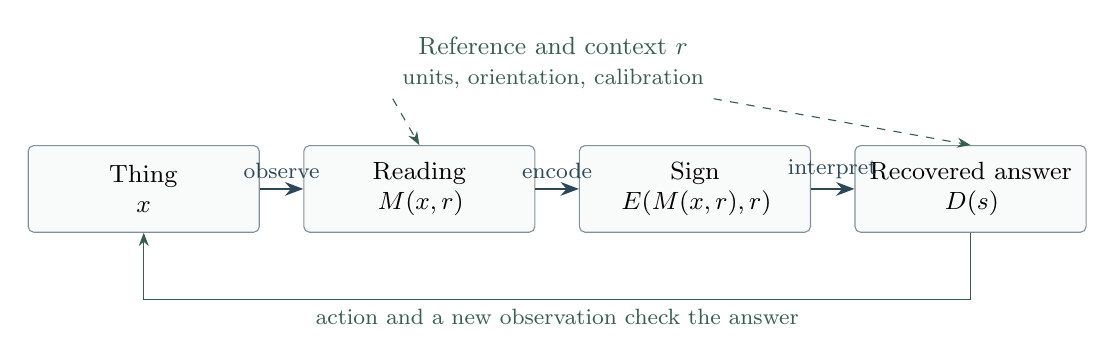
\begin{tikzpicture}[>=Stealth, every node/.style={font=\small},
 box/.style={draw=inkblue!60,rounded corners=2pt,minimum height=11mm,
 text width=27mm,align=center,fill=inkblue!3}]
\node[box] (x) at (0,0) {Thing\\$x$};
\node[box] (y) at (3.5,0) {Reading\\$M(x,r)$};
\node[box] (s) at (7,0) {Sign\\$E(M(x,r),r)$};
\node[box] (a) at (10.5,0) {Recovered answer\\$D(s)$};
\draw[->,inkblue,thick] (x)--node[above,font=\footnotesize]{observe}(y);
\draw[->,inkblue,thick] (y)--node[above,font=\footnotesize]{encode}(s);
\draw[->,inkblue,thick] (s)--node[above,font=\footnotesize]{interpret}(a);
\node[align=center,text=inkgreen] (r) at (5.2,1.6)
 {Reference and context $r$\\\footnotesize units, orientation, calibration};
\draw[->,inkgreen,dashed] (r.south west)--(y.north);
\draw[->,inkgreen,dashed] (r.south east)--(a.north);
\draw[->,inkgreen] (a.south)--++(0,-.85)-|node[pos=.25,below,font=\footnotesize]
 {action and a new observation check the answer}(x.south);
\end{tikzpicture}

\caption{The paper follows a relationship through observation, representation
and response. Calibration makes the observation interpretable; a reference and
a check make the receiver's response comparable with what was intended.}
\label{fig:chain}
\end{figure}

\subsection{A note on interdisciplinarity}
I came to the question from psychology: how can two people know that they have
understood one another? Asking for a definition produces another description;
asking them to do something with the description gives us an outcome to compare.
Following that comparison reaches measurement, and following measurement reaches
the relationships that make a reading repeatable.

The disciplines therefore enter through a common problem. A physical record
must be realized somewhere, as Landauer emphasizes \citep{Landauer1996}; a
mathematical description must specify its objects and operations; a psychological
account must explain what a person can do with a relation they have learned.
Keeping those obligations together is the method of this paper. The circle
will provide a case simple enough to follow through every step, before we ask
how its comparison extends to richer objects.

\section{A communication problem}
\label{sec:communication}

As soon as I know something and set out to tell you, we have a communication
problem. The word \emph{bank} can reach you perfectly while leaving open whether
I mean a financial institution or the edge of a river. The signal arrived;
understanding it calls on the setting in which it was used. Here we are also
using language to discuss language, so the question returns: how do I convey
information about information?

Weaver separates three questions in his introduction to Shannon's theory
\citep{Weaver1949}. Level A concerns the accuracy of transmission. Level B
concerns whether the symbols convey the intended meaning. Level C concerns
whether that meaning leads to the intended effect. A person can repeat a
sentence without understanding its use, and can understand a request while
choosing a different action. Each level needs its own observation.

The present inquiry concerns Level B and the way it can be checked through
Level C. In this semantic use, information is what remains available across
different expressions: the lighter reached through \emph{lighter} and
\emph{igniter}, or one rotation described in degrees and radians. Communication
requires enough agreement that what I mean can become what you understand.
Mathematical language makes that agreement exact by specifying what its
symbols denote and what operations on them do.

Frege's contrast between $a=a$ and $a=b$ helps explain why sameness can teach us
something \citep{Frege1892}. Learning that the morning star and the evening star
are Venus adds a route between descriptions of the same object. The object
does not have to change for the reader's knowledge to change. A successful
message connects a new description to something that can be recognized.

\begin{formal}{F02}{The semantic round trip}{definition and exact recovery criterion}
Let $A$ be the set of meanings relevant to a specified task, $S$ a set of
messages, and $E:A\to S$, $D:S\to A$ an encoder and decoder with a shared
interpretation. Exact semantic recovery is
\begin{equation}\label{eq:roundtrip}
 D(E(a))=a\qquad\text{for every }a\in A.
\end{equation}
Consequently $E$ is injective: if $E(a)=E(b)$, applying $D$ gives $a=b$.
Different signs may still decode to one meaning, because $D$ need not be
injective. Thus \emph{lighter} and \emph{igniter} may have the same decoded value.

When a context $r$ determines interpretation, use $E_r$ and $D_r$. A technical
channel $C$ may satisfy $C(s)=s$ while a receiver uses $D_{r'}$ with $r'\ne r$;
then $D_{r'}(C(E_r(a)))$ can differ from $a$. This is the mathematical shape of
the bank example. The condition states what successful communication means
after the task and interpretations have been specified.
\end{formal}

If the instruction is to rotate a pointer through a quarter cycle, one person
can write $90^\circ$, another $\pi/2$, and another multiplication by $i$.
Reading the numeral $90$ as radians sends the pointer elsewhere even if every
character crossed the channel intact. A return test compares the resulting
rotation with the intended one. This is where the identity principle becomes
an operation: we carry out a transformation and check what it preserved.

\begin{formal}{F03}{Preserving an operation as well as a name}{representation criterion}
Let $T:X\to X$ be an allowed transformation and $E:X\to Z$ a representation.
Let $\widehat T:Z\to Z$ denote the represented operation. The required agreement is
\begin{equation}\label{eq:equivariance}
 E(Tx)=\widehat T(E(x)).
\end{equation}
This is equivariance: performing the operation before or after encoding gives
the same represented result. For degrees and radians,
$E(\theta)=\pi\theta/180$ converts the units, and adding $90$ degrees becomes
adding $\pi/2$ radians.

Together, \eqref{eq:roundtrip} and \eqref{eq:equivariance} say what a usable
translation must retain: the relevant answer and the operations that make it
useful. They also provide a way to test a learned representation without
judging it only by resemblance between its symbols.
\end{formal}

\section{Shannon's bit}
\label{sec:shannon}

How did Shannon make the communication problem manageable? He began with the
messages that could be selected and asked how reliably their selection could
be reproduced elsewhere. Meaning was set aside because the engineering system
had to work for whatever interpretation the users assigned to those messages
\citep{Shannon1948}. Weaver explains the measure as belonging to the situation
of choice, rather than to the significance of a particular utterance
\citep{Weaver1949}.

His example makes the distinction easy to see. Suppose the two possible
messages are the whole King James Bible and the single word ``Yes''. If both
ends already possess the alternatives and their code, one signal selects either
of them. The receiver can use $0$ for the first and $1$ for the second. The
choice can be small even when the selected object is large, because the
description needed to identify that object has already been shared.

The bit counts this choice between two equally likely alternatives as one.
Adding another independent binary choice doubles the possibilities, and two
bits distinguish four outcomes. Three distinguish eight. The logarithm enters
because the number of combinations multiplies while the number of choices
adds. Unequal probabilities then refine the count: an outcome we expected
with certainty resolves nothing, while an unlikely outcome resolves more.

\begin{formal}{F04}{Choice, probability and repetition}{established information theory}
For a discrete random message $X$ with probabilities $p(x)$, define
\begin{equation}\label{eq:entropy}
 I(x)=-\log_2p(x),\qquad H(X)=-\sum_xp(x)\log_2p(x).
\end{equation}
Here $I(x)$ is the information associated with an outcome and $H(X)$ its
expected value. For $N$ equally likely messages, $H(X)=\log_2N$.
Independent choices satisfy $H(X,Y)=H(X)+H(Y)$; in general,
\begin{equation}\label{eq:chain-entropy}
 H(X_1,\ldots,X_n)=\sum_{k=1}^n H(X_k\mid X_1,\ldots,X_{k-1}).
\end{equation}
Shannon develops these properties and their coding interpretation
\citep{Shannon1948}.

A source known to send only $0$ has $H=0$, and the same is true of a source
known to send only $1$. If the source first chooses fairly between $000000$
and $111111$, the whole message contains one bit, despite its repetition.
Independent fair symbols contain one bit each, including a realized run of
zeros. These examples make the relationship precise: information depends on
which possibilities could have occurred and which remain after observation.
The appearance of a mixed string alone does not determine its entropy.
\end{formal}

Binary gains its reach by combining symbols with position. In $1101$, the
positions carry weights $8,4,2,1$, so the numeral represents thirteen. Numbers
can then index letters, colour levels or sound samples. Each use has a
reference: an alphabet, a pixel arrangement, a clock, a unit. What can be sent
depends on the distinctions those references make available.

Every physical bit also occupies a physical state, such as two voltage ranges
or two magnetization directions. To draw the distinction geometrically, put
two marks one unit apart. With two bits, let each vary while the other remains
fixed: the four possibilities become the corners of a square. Three bits make
a cube, and further bits give its higher-dimensional versions. Boolean
analysis already works directly on this geometry \citep{ODonnell2014}.

\begin{formal}{F05}{The binary cube and its operations}{established construction}
For $n$ labelled positions the state set is $\{0,1\}^n\subset\R^n$, with
the usual orthonormal coordinate basis. Two strings $x,y$ have Hamming distance
\begin{equation}
 d_H(x,y)=\sum_{k=1}^n |x_k-y_k|=\|x-y\|_2^2.
\end{equation}
Each coordinate records a separately addressable distinction. For two inputs,
$\operatorname{AND}(x,y)=xy$ and
$\operatorname{XOR}(x,y)=x+y-2xy$ agree with their truth tables at all four
corners. A code corrects up to $t$ bit flips when its minimum distance is at
least $2t+1$ \citep{Hamming1950}.

This is a geometric representation with a chosen metric. Coordinate
orthogonality expresses separation of readings; probabilistic independence is
an additional property of a distribution. The ordered strings $01$ and $10$
remain different corners. Binary coding can therefore preserve order when its
positions preserve it.
\end{formal}

Noise changes what arrives. A scratch may flip a bit, and a weak signal may
leave two alternatives hard to distinguish. Shannon asks how much information
can pass reliably through a specified channel, allowing long codes to protect
the choices. This question remains part of the present theory: giving a
meaning a geometric representation still leaves us with a physical channel
through which that representation must travel.

\begin{formal}{F06}{Capacity and the continuous channel}{established results with their models}
For a discrete memoryless channel $p(y\mid x)$, capacity per channel use is
\begin{equation}
 C=\max_{p(x)} I(X;Y),\qquad I(X;Y)=H(X)-H(X\mid Y).
\end{equation}
Rates below capacity admit arbitrarily small decoding error with sufficiently
long suitable codes. This statement depends on the channel model and coding
assumptions. For an ideal real band-limited additive white Gaussian noise
channel of bandwidth $B$, average signal power $P$ and noise power $N$ in the
band, the corresponding rate is
\begin{equation}
 C=B\log_2(1+P/N)\quad\text{bits per second}.
\end{equation}
Gaussian noise is this particular continuous example, not an assumption of
all Shannon theory \citep{Shannon1948,Shannon1949}.

For a signal whose Fourier transform vanishes outside $[-B,B]$, suitable
sampling at interval $1/(2B)$ reconstructs it through
\begin{equation}\label{eq:sampling}
 f(t)=\sum_{k\in\Z} f\left(\frac{k}{2B}\right)
 \operatorname{sinc}(2Bt-k),\quad
 \operatorname{sinc}(u)=\frac{\sin(\pi u)}{\pi u},
\end{equation}
under the usual bandlimit and convergence hypotheses. The samples retain
phase and structure when the model and clock are known. A time window $T$ has
roughly $2BT$ effective real degrees of freedom; exact simultaneous compact
time support and band support are different requirements.
\end{formal}

The first part of the story is now in place. A bit counts alternatives,
entropy measures uncertainty over them, and a channel limits reliable
transmission. The alternatives themselves must already be identifiable. The
question for meaning is how to carry and check the relationships that let a
receiver identify them after the description changes.

\section{The geometric bit}
\label{sec:geometric}

What is the shape of a comparison that keeps its reference? Draw a circle and
mark a point on it. Draw the diameter through that point and a second diameter
at a right angle. The construction gives four positions before we name them:
the starting point, its opposite, and the two positions halfway between.
Writing $1,i,-1,-i$ records the quarter rotations that relate them.

Perpendicularity distinguishes two directions while preserving the unit used
to compare them. Symmetry relates opposite positions through the same
half-rotation. Follow the marked point around the boundary and its position
changes continuously, while the radius and the relationships between the axes
remain fixed. After a full rotation the point reaches its start. We can now
show sameness through a change, carry out a comparison, and measure a failure
to return.

This is the paper's answer to the question with which we began:
\emph{information is invariance over change}. The geometric bit gives that
answer a form we can operate. It is the circular relationship together with a
reference and a comparison, so that identity is available as a check. The
principle $A=A$ becomes something we can perform through a representation,
transform and return, rather than leave implicit in the name of an alternative.

\subsection{The alphabet of the circle}
The alphabet of binary is $0$ and $1$, and DNA uses four bases in sequences
whose organization matters to their function. Here the alphabet is relational:
perpendicularity and symmetry. They describe how one direction differs from
another and how the same relation appears again. The symbols enter after the
construction, as a concise way of carrying it.

Why does $i$ appear? A quarter rotation applied twice reaches the opposite;
applied four times it returns. On the plane, the operation sending a horizontal
unit vector to a vertical one therefore has a square equal to negation.
Writing that operation as $i$ gives $i^2=-1$. The expression is a record of
what the operation does.

\begin{formal}{F07}{From the right angle to Euler's formula}{elementary derivation}
On an oriented Euclidean plane choose an orthonormal basis and define
\begin{equation}
 J=\begin{pmatrix}0&-1\\1&0\end{pmatrix},\qquad
 J^2=-I,\qquad J^\mathsf{T}=-J.
\end{equation}
For a unit initial vector $v_0$, the differential equation
$v'(\theta)=Jv(\theta)$ has solution
\begin{equation}\label{eq:euler}
 v(\theta)=e^{\theta J}v_0
 = (I\cos\theta+J\sin\theta)v_0.
\end{equation}
The last equality follows by grouping the even and odd powers in the
exponential series. Moreover,
$\frac{\mathrm d}{\mathrm d\theta}\|v\|^2
=2v^\mathsf{T}Jv=0$, so the solution remains on the unit circle.
Identifying $J$ with multiplication by $i$ gives
\begin{equation}
 e^{i\theta}=\cos\theta+i\sin\theta,\qquad
 e^{i\pi}=-1,\qquad e^{2\pi i}=1.
\end{equation}
The exponential accumulates the generator; the generator $i$ makes that
change perpendicular. The half-period $\pi$ reaches the opposite. Thus the
presentation's descriptions of $e$ as accumulation and $\pi$ as symmetry have
precise roles in one equation. Real exponential growth and perpendicular
rotation use different generators of the same exponential construction.
\end{formal}

\begin{figure}[htbp]
\centering
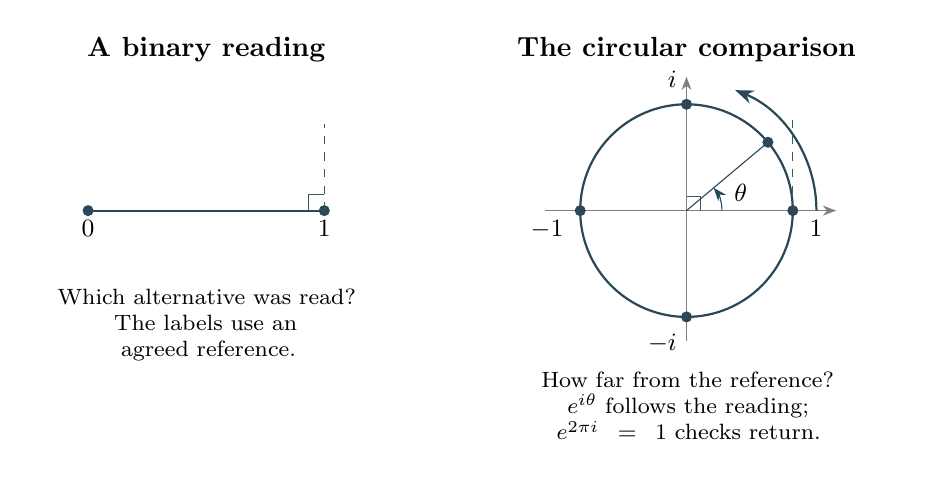
\begin{tikzpicture}[>=Stealth,every node/.style={font=\small}]
\node[font=\bfseries] at (0,2.05) {A binary reading};
\draw[thick,inkblue] (-1.5,0)--(1.5,0);
\fill[inkblue](-1.5,0)circle(2pt) (1.5,0)circle(2pt);
\node[below]at(-1.5,0){$0$};\node[below]at(1.5,0){$1$};
\draw[dashed,inkgreen] (1.5,0)--(1.5,1.1);
\draw[inkgreen](1.3,0)--(1.3,.2)--(1.5,.2);
\node[align=center,text width=43mm,font=\footnotesize]at(0,-1.45)
 {Which alternative was read?\\The labels use an agreed reference.};
\begin{scope}[shift={(6.1,0)}]
\node[font=\bfseries]at(0,2.05){The circular comparison};
\draw[inkblue,thick](0,0)circle(1.35);
\draw[->,black!50](-1.8,0)--(1.9,0);
\draw[->,black!50](0,-1.65)--(0,1.7);
\draw[inkgreen](.18,0)--(.18,.18)--(0,.18);
\draw[->,inkblue,thick](1.65,0)arc(0:68:1.65);
\draw[dashed,inkgreen](1.35,0)--(1.35,1.15);
\foreach \p/\s/\anchor in {0/1/north west,90/i/south east,180/-1/north east,270/-i/north east}{
 \fill[inkblue](\p:1.35)circle(2pt);
 \node[anchor=\anchor]at(\p:1.44){$\s$};}
\draw[inkblue](0,0)--(40:1.35);\fill[inkblue](40:1.35)circle(2pt);
\draw[->,inkblue](.45,0)arc(0:40:.45);
\node at(.69,.23){$\theta$};
\node[align=center,text width=55mm,font=\footnotesize]at(0,-2.48)
 {How far from the reference?\\$e^{i\theta}$ follows the reading; $e^{2\pi i}=1$ checks return.};
\end{scope}
\end{tikzpicture}

\caption{A discrete reading retains an alternative; the circular comparison
also retains the reference and the operation relating readings. The two axes
are perpendicular, the opposite poles are symmetric, and rotation preserves
the circle. The radius and tangent at a point are perpendicular as well.}
\label{fig:unit}
\end{figure}

\subsection{A unit that can be checked}
The circle brings together a continuous path and a countable event. Its
boundary can be followed continuously, while a completed rotation can be
counted as one. When we cut a pizza into four equal quarters, the right angles
belong to that construction before we assign numbers to the pieces. Choosing
the first cut sets the orientation; making its perpendicular sets the other
axis. Rotating the whole arrangement changes neither the quarters nor their
relations.

The useful distinction is between the relation and its reading. We may record
only which half contains the mark, record a quadrant, or measure an angle to a
chosen precision. Each answer is a different description of the same comparison
space. A finite alphabet becomes available by deciding which differences the
reading must preserve.

\begin{formal}{F08}{The geometric bit and its discrete readings}{definition and interpretation}
Define the circular comparison unit as
\begin{equation}\label{eq:unit}
 \mathcal G=(S^1,1,\mu,J,d),\qquad
 S^1=\{z\in\C:|z|=1\},\quad \mu(z,w)=zw,
\end{equation}
where $1$ is the reference, $Jz=iz$ is the quarter rotation, and
\begin{equation}\label{eq:circle-distance}
 d(z,w)=|\Arg(\bar z w)|\in[0,\pi].
\end{equation}
This tuple is the \emph{geometric bit} in this manuscript. Its identity check is
$\bar z w=1$, equivalently $d(z,w)=0$. Its intended semantic role is to give
the identity principle an operational representation.

Choose $\theta\in[0,2\pi)$ and define
$Q_m(e^{i\theta})=\lfloor m\theta/(2\pi)\rfloor$.
For $m=2$ this records a half-circle; for $m=4$ it records a quadrant.
A distribution of readings has Shannon entropy $H(Q_m(Z))$. This construction
recovers binary alternatives as a coarse reading. The circle itself is a
continuum, and ``geometric bit'' names the comparison structure rather than a
claim that an arbitrary angle costs one Shannon bit to transmit.
\end{formal}

Two people facing different directions can compare angles if each keeps the
reference in the same description as the reading. Rotate the reference and
the reading together, and their separation remains unchanged. This is the
smallest complete example of what the lighter asks of us: our views can differ
while a relation survives the change between them.

\begin{formal}{F09}{The reference travels with the reading}{exact invariance}
For reference $r\in S^1$ and reading $z\in S^1$, let
$c(r,z)=\bar r z$. Under a common frame change $u\in S^1$,
\begin{equation}\label{eq:reference}
 c(ur,uz)=\overline{ur}\,uz=\bar r\bar uuz=\bar r z=c(r,z).
\end{equation}
Two observers therefore recover the same relative phase from differently
oriented coordinates. If they transmit only $z$ and omit an unknown $r$,
the value of $c(r,z)$ is generally undetermined. A representation carrying
both a reading and a usable reference solves this particular ambiguity.

For an image or a physical object, the analogous construction needs an
observation model. Sampling reconstructs the band-limited field of
Box~\ref{F06} from sufficient calibrated samples; recovering a three-dimensional
lighter also involves viewpoint, illumination and occlusion. The shared-frame
calculation is exact for its stated circular task and supplies the pattern
that a richer representation must implement.
\end{formal}

\subsection{Closure, counting and uncertainty}
Following a point for one rotation or for two ends at the same place. We have
to keep a count if the distinction between those journeys matters. The circle
then gives two records: where the point is now and how many completed
rotations brought it there. This is the continuous-to-discrete relationship
behind the counting language of the presentation.

Closure also supplies a second question alongside uncertainty. Before the
message arrives, which alternatives remain possible? After interpreting it,
how closely does the result agree with the reference? Entropy answers the
first, and a closure residual answers the second. The thesis treats them as
complementary roles in knowing: a difference is measured against something
that holds, and what holds is recognized through differences.

\begin{formal}{F10}{Endpoint, winding and closure residual}{established topology and defined measurement}
The covering map
\begin{equation}
 p:\R\to S^1,\qquad p(t)=e^{2\pi it},\qquad p^{-1}(1)=\Z
\end{equation}
retains phase while identifying histories that differ by a whole number of
rotations. A continuous path has a unique real lift once its initial lift is
chosen. A closed path then has integer winding
$n=\widetilde\theta(T)-\widetilde\theta(0)$ in turns, expressing
$\pi_1(S^1)\cong\Z$ \citep{LicataShulman2013}.

For expected endpoint $r$ and reconstructed endpoint $z$, define the closure
residual $\varepsilon=d(r,z)$. It is zero exactly when the endpoints agree.
If the task includes winding, compare $(z,n)$ rather than $z$ alone.

Entropy $H(X)$ is measured in bits and depends on a probability distribution;
$\varepsilon$ is measured in radians and depends on a reference. No universal
constant makes their sum fixed. For example, a fair binary message can have
entropy one and be recovered with zero residual on every trial. Closure is
therefore a verification measurement alongside uncertainty, with its own
specified object and unit.
\end{formal}

\section{Identity, measured}
\label{sec:measurement}

What changes once identity is measured instead of assumed? We can ask whether
the relationship in the description is also the relationship an instrument
finds. A string around a circular rim compares circumference with diameter.
A clock compares equal intervals in a decay or oscillation. A plumb line and
a locally level surface make a right angle available to construction. These
are different ways of approaching the constants and operations in Euler's
formula, through things we can do in the world.

The notation is ours to choose. We could name a quarter rotation in degrees,
radians or turns, while the pointer reaches the same place. What the notation
preserves is constrained by the measurement. This is the sense in which the
paper calls Euler's identity a physical law of comparison: its circular
relationship is realized and repeatedly checked by physical operations.

This claim has a mathematical layer and an empirical layer. The exact return
follows in the rotation model; experiments establish how well an apparatus
realizes that model. Holding the layers together gives the law practical
content, because a discrepancy can be assigned to a unit, a reference, a
transformation or an instrument instead of being hidden inside an inscription.

\begin{formal}{F11}{The proposed law of comparison}{physical interpretation with an explicit model}
An ideal circular apparatus realizes a continuous, orientation-preserving
rotation $R(\theta)$ with $R(0)=I$, a fixed Euclidean norm, and a calibrated
angle satisfying $R(\alpha+\beta)=R(\alpha)R(\beta)$. With one revolution
calibrated as $2\pi$, Box~\ref{F07} gives $R(2\pi)=I$ exactly.
An experimental return has residual
\begin{equation}
 \varepsilon_{\rm exp}=d(z_{\rm initial},z_{\rm final}),
\end{equation}
reported with uncertainty from resolution, drift and calibration. Reproducing
this relation across instruments is the empirical content of the proposed
law. Its exact mathematical content belongs to the stated rotation model.

The circumference test assumes Euclidean planar geometry. On a sphere of
radius $a$, a geodesic circle of radius $s$ has circumference
$2\pi a\sin(s/a)$, giving the ratio
$\pi\sin(s/a)/(s/a)$ to $2s$. Local flatness recovers $\pi$ as $s/a\to0$.
The phase identity remains exact while the metric interpretation of a
particular circumference changes. A measurement must specify which circle and
which distance it compares.
\end{formal}

\subsection{Why the same equation keeps appearing}
Let change be proportional to what is already present and the exponential
appears. Let that change point along the present state and it grows or
decays; let it point perpendicularly and it rotates. A charged capacitor and
a rotating phase therefore use the same accumulation rule with different
generators. The numerical value of $e$ belongs to the normalized exponential,
while the physical rate tells us how laboratory time enters its exponent.

In mechanics, the oscillator moves around its energy contours. In quantum
mechanics, unitary evolution keeps the length of the state vector. In signal
processing, sines and cosines let a field be resolved into components whose
amplitude and phase can be measured. These are substantial instances of the
same geometric language. Each obtains its physical prediction from a generator
and a model, as well as from the exponential that composes their effects.

\begin{formal}{F12}{Three concrete realizations}{established dynamics}
For $\dot x=kx$, $x(t)=x(0)e^{kt}$, where $k$ has units of inverse time. For
the harmonic oscillator, take normalized coordinates
$Q=\sqrt{m\omega}\,q$ and $P=p/\sqrt{m\omega}$, and let $z=Q+iP$.
Hamilton's equations give
\begin{equation}
 \dot z=-i\omega z,\qquad z(t)=e^{-i\omega t}z(0).
\end{equation}
The energy is proportional to $|z|^2$, so it remains fixed during rotation.
More generally, canonical Hamiltonian evolution has
$\dot x=J\nabla H$, with antisymmetric $J$, and
$\dot H=(\nabla H)^\mathsf{T}J\nabla H=0$ for a time-independent Hamiltonian.

For a finite-dimensional closed quantum system with self-adjoint Hamiltonian
$\widehat H$, Schr\"odinger evolution is
\begin{equation}
 i\hbar\dot\psi=\widehat H\psi,\qquad
 \psi(t)=e^{-it\widehat H/\hbar}\psi(0).
\end{equation}
It preserves $\langle\psi,\psi\rangle$ because the generator is skew-Hermitian.
The velocity is perpendicular to the state in the real inner product
$\Real\langle\cdot,\cdot\rangle$; it need not be orthogonal in the complex
inner product. Several incommensurate eigenfrequencies need not return together
after a finite time. These statements explain precisely which rotation
properties the physical examples share.
\end{formal}

The same distinction helps with conservation. Noether connects continuous
symmetries of an action with conserved quantities under definite variational
conditions \citep{Noether1918}. The circle offers a simple symmetry we can
operate, while a conservation law also needs the dynamics to which that
symmetry applies. Similarly, entropy needs a statistical model of alternatives;
perpendicular axes provide a representation in which separate variations can
be described. The thesis brings these roles into one comparison rather than
treating the words as interchangeable equations.

\subsection{What counts as a check?}
To exist physically, in the operational account used here, is to be available
to interaction. The lighter reflects light, exchanges heat, rests on the desk
and resists a hand. Those relationships continue when we look away. The
observer, the instrument and the inscription participate in the same world,
so the description can be brought back to a comparison outside its own wording.

That is the epistemological use of consistency in this argument. Agreement
between independent procedures strengthens the case that they preserve a
common relationship. A string, a clock and an optical phase measurement can
constrain the same model from different directions. Their agreement motivates
the unifying interpretation; each observation still has a domain and a
precision that can be examined by another person.

\begin{formal}{F13}{Operational identity and the scope of verification}{methodological definition}
Fix a family of admissible observations $\mathcal M$. Define
\begin{equation}\label{eq:operational-equivalence}
 x\sim_{\mathcal M}y\quad\Longleftrightarrow\quad
 M(x)=M(y)\ \text{for all }M\in\mathcal M.
\end{equation}
For stochastic observations, require equality of their outcome distributions.
This is an equivalence relation, and the quotient $X/{\sim_{\mathcal M}}$
records precisely the distinctions those observations can resolve. Enlarging
$\mathcal M$ can separate previously equivalent states.

An invariant $f(Tx)=f(x)$ preserves identity relative to allowed transformations
$T$; a \emph{complete} invariant additionally distinguishes the equivalence
classes relevant to the task. A circle's constant radius is an invariant,
but radius alone does not identify an arbitrary physical object.

Formal verification and empirical checking address different parts of the
chain. G\"odel's incompleteness theorems concern consistent, effectively
axiomatized systems of sufficient arithmetic strength \citep{Godel1931}.
External measurements give scientific models new evidence; they do not remove
those hypotheses or convert every true statement into a formal proof. Here
the evidence, the formal implication, and the interpretation are each made
available for inspection.
\end{formal}

The thesis is now explicit: the identity that supports communication is a
relationship preserved through interaction and transformation, and geometry
gives us an apparatus for measuring it. The circular construction establishes
this directly for rotational comparisons. To understand what richer objects
require, we next compose those comparisons and keep track of what survives.

\section{Operating geometric bits}
\label{sec:operations}

What can geometric bits do, and where do they stop? Shannon's theory gives a
unit, a measure, rules for composing messages and limits on a channel. With
the reference retained, the same questions become questions about a comparison
that can be composed and checked. We need to know which structure composition
preserves, how much a description keeps, and what a discrepancy tells us.

\begin{table}[htbp]
\centering\small
\begin{tabularx}{\linewidth}{@{}p{22mm}XX@{}}
\toprule
Question & Shannon's quantitative account & Geometric comparison developed here\\
\midrule
Unit & A bit of uncertainty & A referenced circular comparison\\
Measure & Entropy and mutual information & Relative phase and closure residual, alongside entropy\\
Composition & Ordered strings and joint signal spaces & Joint states and ordered algebraic products\\
Limit & Capacity of a specified channel & Norm-preserving algebraic composition under Hurwitz's hypotheses\\
Noise & Error probabilities and recoverable rate & Exact single-factor transport and aligned local discrepancies\\
Meaning & Interpretation supplied by the task & Interpretation and its verification included in the protocol\\
\bottomrule
\end{tabularx}
\caption{The theories answer connected questions at different points of the
communication chain. A geometric representation continues to incur coding,
calibration and channel costs.}
\label{tab:comparison}
\end{table}

\subsection{Side by side, and in sequence}
There are two operations to distinguish at the outset. Put two rotations side
by side and we can describe both at once. Let one operation act after another
and their order can change the result. A photograph uses many sampled values
side by side; rotating a camera successively about two different axes is an
ordered composition. Both carry information, and each preserves different
relationships.

Holding a list of complex amplitudes to one total norm gives a sphere. Two
complex amplitudes supply four real coordinates with one norm constraint, so
their unit states lie on the three-sphere. This is also the unit sphere of
quaternions, which supplies an additional operation: multiplying one unit
quaternion by another. The shared sphere lets the two descriptions meet;
the multiplication tells us how to operate its points.

\begin{formal}{F14}{Three composition spaces}{established constructions}
For $m$ phases with each amplitude fixed, the joint space is the torus
$(S^1)^m$. Allowing the amplitudes to vary while fixing their total squared
norm instead gives
\begin{equation}\label{eq:sphere}
 \left\{(z_1,\ldots,z_m)\in\C^m:
 \sum_{j=1}^m|z_j|^2=1\right\}=S^{2m-1}.
\end{equation}
Here $z_j=r_je^{i\theta_j}$, with $\sum r_j^2=1$. The phase of a zero
component has no effect. A common phase acts by $z\mapsto e^{i\alpha}z$;
its quotient is complex projective space $\mathbb{CP}^{m-1}$.

For $m=2$, identify the same four real coordinates with
$q=w+xi+yj+zk\in\HH$, $|q|=1$. Ordered composition uses Hamilton's rule
\begin{equation}\label{eq:hamilton}
 (a,\mathbf u)(b,\mathbf v)=
 (ab-\mathbf u\!\cdot\!\mathbf v,
 a\mathbf v+b\mathbf u+\mathbf u\!\times\!\mathbf v).
\end{equation}
This operation keeps the norm and retains order. The dot and cross products
are the scalar and vector contributions of one multiplication. A normalized
list, a torus of fixed phases and an ordered product are thus three explicit
constructions, rather than three names for one unspecified composition.
\end{formal}

To see what order adds, rotate a physical frame about one axis and then
another. Interchanging the rotations changes where the frame points. Complex
phases compose by adding angles and therefore commute, while quaternionic
rotations record the difference between the two orders. Perpendicularity now
enters the multiplication itself, through the cross product.

\subsection{The algebraic limit and the nested fibrations}
How far can this construction grow while multiplying lengths exactly? The
question has a sharp mathematical answer once its requirements are stated.
Over the reals, the finite-dimensional unital algebras with a positive
multiplicative norm occur in dimensions one, two, four and eight. They are
the real numbers, complex numbers, quaternions and octonions. This is
Hurwitz's classification, presented with its geometric consequences by
\citet{Baez2002}.

The succession matters because each level can carry the previous one. A
chosen complex plane still rotates by Euler's formula inside the quaternions
or octonions. New independent directions enrich composition while preserving
that local comparison. At the same time, the operation changes: quaternions
give up commutativity, octonions give up associativity, and the next
Cayley--Dickson doubling loses the multiplicative norm.

\begin{formal}{F15}{The limit theorem used in this paper}{established classification}
Let $A$ be a finite-dimensional real algebra with identity, bilinear
multiplication and a positive-definite quadratic norm satisfying
\begin{equation}\label{eq:multiplicative-norm}
 |ab|=|a|\,|b|\qquad\text{for every }a,b\in A.
\end{equation}
Then $A$ is isomorphic to $\R,\C,\HH$ or $\OO$, of real dimensions
$1,2,4,8$. The octonions are alternative: every two elements generate an
associative subalgebra. The theorem concerns this specified algebraic class.
Arbitrarily large vector spaces, matrix algebras, tensor products and composite
quantum systems remain available outside it.

Norm preservation also preserves perpendicularity. For a unit $a$, the map
$L_a:x\mapsto ax$ is real-linear and preserves lengths. By polarization,
\begin{equation}
 \langle ax,ay\rangle
 =\tfrac12\bigl(|a(x+y)|^2-|ax|^2-|ay|^2\bigr)
 =\langle x,y\rangle.
\end{equation}
The same holds for right multiplication. This is the exact content of
preserving sameness of length and difference of direction during composition.
\end{formal}

The associated Hopf maps organize observation as well as composition. A
normalized pair determines a relative description, while a whole sphere of
states shares that description. What we read is the base; what it leaves
unresolved is the fibre. The previous level's full state space reappears as
the next level's fibre type. This is the recursive structure meant here by
the fractality of the object: the comparison recurs inside a richer one.

\begin{formal}{F16}{One rule for the four Hopf maps}{established bundles and explicit compatibility}
For $A=\R,\C,\HH,\OO$, let $n=\dim_\R A$ and
$|a|^2+|b|^2=1$. Define
\begin{equation}\label{eq:hopf}
 h_A(a,b)=(|a|^2-|b|^2,\,2a\bar b)\in\R\oplus A.
\end{equation}
The norm identity gives
\begin{equation}
 \|h_A(a,b)\|^2=(|a|^2-|b|^2)^2+4|a|^2|b|^2=1.
\end{equation}
These are the division-algebra Hopf fibrations, with the sphere fibres shown
in Table~\ref{tab:hopf} \citep{Baez2002}. Their nontrivial sphere-over-sphere
pattern is tied to the Hopf-invariant-one theorem \citep{Adams1960}.

Let $j:A\hookrightarrow B$ be one of the standard norm- and
conjugation-preserving inclusions. With
$J(a,b)=(j(a),j(b))$ and $K(t,x)=(t,j(x))$, substitution proves
\begin{equation}\label{eq:hopf-compatibility}
 h_B\circ J=K\circ h_A.
\end{equation}
The larger projection retains the smaller one exactly. If $D(A)=A\oplus A$
is the next doubling for $A=\R,\C,\HH$, then
\begin{equation}
 h_{D(A)}^{-1}(1,0)=\{(q,0):|q|=1\}\cong S(A^2).
\end{equation}
Thus the previous total space is exactly a distinguished next fibre. Other
fibres require a chosen identification to carry that prior structure.

This is a finite structural recurrence. The next formula fails with sedenion
multiplication: choose nonzero zero divisors $xy=0$ with
$|x|=|y|=1/\sqrt2$, and set $a=x$, $b=\bar y$. Then the normalized input
maps to $(0,0)$ rather than to a unit sphere. The octonionic map already has
total space $S^{15}$; it remains valid because its formula uses octonionic
multiplication. An octonionic fibre $S^7$ is not an associative phase group.
\end{formal}

\begin{table}[htbp]
\centering
\begin{tabular}{@{}lcccl@{}}
\toprule
Algebra & Real dimension & Fibre & Total space & Base\\
\midrule
$\R$ & 1 & $S^0$ & $S^1$ & $S^1$\\
$\C$ & 2 & $S^1$ & $S^3$ & $S^2$\\
$\HH$ & 4 & $S^3$ & $S^7$ & $S^4$\\
$\OO$ & 8 & $S^7$ & $S^{15}$ & $S^8$\\
\bottomrule
\end{tabular}
\caption{The same normalized comparison rule at four algebraic levels. Reading
downward, each total-space type becomes the next fibre type. Reading across,
projection retains a relative description while a fibre remains unresolved.}
\label{tab:hopf}
\end{table}

Binary is already inside this algebra. Label the quaternion units $1,i,j,k$
by $00,01,10,11$. Multiplication combines their bit labels by XOR and retains
an additional sign. Since $ij=k$ and $ji=-k$, that sign records the difference
between the two orders. This supplies a precise bridge between the cube and
the sphere, without asking a reader to accept their resemblance as evidence.

\begin{formal}{F17}{Bit strings with an orientation sign}{established algebra and its interpretation}
The eight elements $Q_8=\{\pm1,\pm i,\pm j,\pm k\}$ form a group.
Its commutator subgroup is $\{\pm1\}$, since $[i,j]=-1$, while quotienting
by these signs makes the generators commute. Hence
\begin{equation}\label{eq:q8}
 Q_8/\{\pm1\}\cong\Z_2\times\Z_2.
\end{equation}
In the chosen labels the basis multiplication has the form
$e_ae_b=\epsilon(a,b)e_{a\oplus b}$, with $\epsilon(a,b)\in\{\pm1\}$.
Related twisted group-algebra constructions extend this description to the
octonions \citep{AlbuquerqueMajid1998}.

Equation~\eqref{eq:q8} forgets the sign information carried by quaternion
multiplication. An ordinary binary representation can still encode the full
signed units and their order. The thesis's claim that a binary reading is a
projection is exact for this quotient; it is not a restriction on the
expressive power of binary computers.
\end{formal}

\subsection{What the higher geometry gives the physical argument}
The cup provides the intuition. A circular rim is visible from one direction,
an ellipse from another, and a side view hides much of the interior. Moving
around the cup changes the projection while offering more constraints on one
object. In the algebraic model, the base and fibre make such retained and
unresolved relationships explicit. A projection can be generated from a
richer state even when the projected reading alone cannot recover that state.

Quaternions add three imaginary directions to a scalar component and compose
spatial rotations without leaving their unit sphere. This makes them especially
useful for the $3+1$ discussion. A physical spacetime description also has to
account for its Lorentzian metric, where the time contribution and spatial
contributions have opposite signs. The matrix representation below makes that
extra structure explicit rather than leaving it inside the dimensional count.

\begin{formal}{F18}{Rotation, spacetime and observed quantum states}{established representations; dimensional interpretation}
For a unit quaternion $q=\cos(\theta/2)+\mathbf n\sin(\theta/2)$, conjugation
$v\mapsto qv\bar q$ rotates the imaginary three-space by $\theta$.
The elements $q$ and $-q$ give the same spatial rotation, yielding the double
cover $\SU(2)\to\SO(3)$. Quaternion norm is Euclidean:
$|q|^2=w^2+x^2+y^2+z^2$.

Minkowski coordinates instead form a Hermitian matrix
\begin{equation}
 X=ctI+x\sigma_x+y\sigma_y+z\sigma_z,
 \qquad \det X=c^2t^2-x^2-y^2-z^2.
\end{equation}
For $A\in\mathrm{SL}(2,\C)$, $X\mapsto AXA^\dagger$ preserves this
determinant. Pauli matrices connect this representation with the complexified
quaternion algebra. The signature is essential to its spacetime interpretation.

A normalized qubit $(a,b)\in\C^2$ lies on $S^3$. Its global phase quotient
is the Bloch sphere $\mathbb{CP}^1\cong S^2$, the complex Hopf base. An outcome
along a detector axis $\mathbf n$ has probability
$(1+\mathbf r\cdot\mathbf n)/2$ by the Born rule, where $\mathbf r$ is the
Bloch vector. Passing to the Bloch vector removes global phase; a subsequent
measurement produces an outcome. They are distinct operations.

Poincar\'e--Bendixson restricts compact limit sets of suitable smooth autonomous
planar flows: a nonempty omega-limit set without equilibria is a periodic
orbit \citep{Sideris2013}. Three-dimensional flows can have richer recurrent
dynamics. This supports the paper's dimensional motivation, while neither it
nor the quaternion coordinate count alone derives the dimension of spacetime.
\end{formal}

Other connections belong here because they show what the same constructions
already do. A periodic wave on a ring admits integer winding; bound-state
spectra depend on boundary conditions and the operator whose eigenfunctions
fit them. Two periodic motions at a rational frequency ratio return together,
which can be heard as an interval and drawn as a closed Lissajous curve.
Their lifts to suitable tori give a further topological description. These
are concrete ways in which numbers, sounds and physical motions can be readings
of one specified structure.

At the larger scale, division-algebra research constructs particle
representations related to the Standard Model \citep{Furey2016}. Division
algebras also explain the dimensions $3,4,6,10$ in certain classical
supersymmetric constructions \citep{BaezHuerta2009}. That dimension list has
a different role from the quantum critical dimension of a string theory.
The paper's synthesis is that such recurring structures belong to one
architecture of comparison and composition. Deriving a particular field
content, action or particle spectrum still requires the corresponding physical
construction. The common object is a research claim about those connections,
and the Hopf recurrence states its mathematical core.

\subsection{An exact account of a changed factor}
Suppose a message is represented by an ordered sequence of unit rotations.
Compose them, retain the successive products, and compare the record with a
second sequence. What happens to a small change near the beginning? Unit
multiplication carries it through without changing its size. A later position
has the same sensitivity as an earlier one because both are compared through
isometries.

This is useful in a way that a final verdict of ``different'' is not. We can
measure the discrepancy, return to the local comparison, and ask whether a
factor is absent or has changed position. The distinction has an exact
algebraic form when a single elementary incident has been aligned.

\begin{formal}{F19}{Exact propagation and uniform sensitivity}{derivation from multiplicative norm}
Let $g_1,\ldots,g_n$ be unit quaternions and
$P_k=g_1\cdots g_k$, with $P_0=1$. Replace only $g_k$ by $g'_k$ and
hold all other factors fixed. Write $L=g_1\cdots g_{k-1}$ and
$R=g_{k+1}\cdots g_n$. Associativity gives
\begin{equation}\label{eq:propagation}
 P_n-P'_n=L(g_k-g'_k)R,\qquad
 |P_n-P'_n|=|g_k-g'_k|.
\end{equation}
Both $L$ and $R$ are units, so the second equality follows from
\eqref{eq:multiplicative-norm}. Their real-linear action also preserves inner
products, giving equality of the spherical distances before and after
propagation. The differential $v\mapsto LvR$ is an isometry at every position.
This is uniform sensitivity to one varied factor, with the others fixed.

Stored prefixes recover each factor exactly by
$g_k=\bar P_{k-1}P_k$. For one nonzero substitution with common indexing,
the predicate $P_j=P'_j$ is true before $k$ and false thereafter. Binary
search therefore locates $k$ in $\lceil\log_2n\rceil$ comparisons, given
random access to exact stored prefixes. Constructing and storing them costs
$O(n)$, and the claim counts comparisons, not the bit cost of arbitrary
precision arithmetic. Multiple changes can make prefixes separate and rejoin.
\end{formal}

\begin{figure}[htbp]
\centering
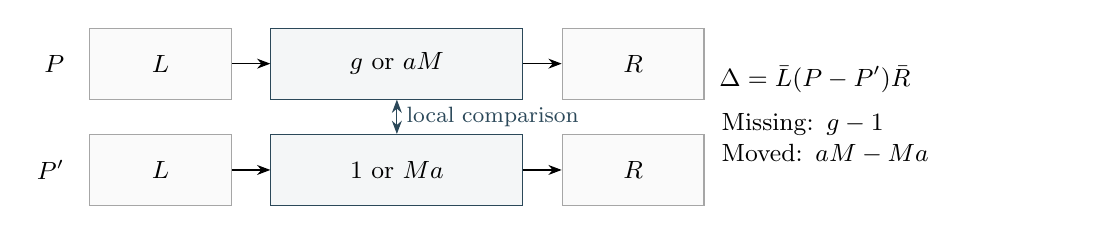
\begin{tikzpicture}[>=Stealth,every node/.style={font=\small},
 ctx/.style={draw=black!35,fill=black!2,minimum width=18mm,minimum height=9mm},
 edit/.style={draw=inkblue,fill=inkblue!5,minimum width=32mm,minimum height=9mm}]
\node[ctx](l)at(0,0){$L$};\node[edit](a)at(3,0){$g$ or $aM$};
\node[ctx](r)at(6,0){$R$};
\node[ctx](ll)at(0,-1.35){$L$};\node[edit](b)at(3,-1.35){$1$ or $Ma$};
\node[ctx](rr)at(6,-1.35){$R$};
\draw[->](l)--(a);\draw[->](a)--(r);
\draw[->](ll)--(b);\draw[->](b)--(rr);
\node[anchor=east]at(-1.1,0){$P$};\node[anchor=east]at(-1.1,-1.35){$P'$};
\draw[<->,inkblue](a)--node[right,font=\footnotesize]{local comparison}(b);
\node[align=left,anchor=west,text width=44mm]at(7,-.65)
 {$\Delta=\bar L(P-P')\bar R$\\[5pt]
 Missing: $g-1$\\Moved: $aM-Ma$};
\end{tikzpicture}

\caption{Remove the common context before classifying an elementary incident.
An insertion leaves $g-1$ in the local frame; a move leaves $aM-Ma$. The
context changes the appearance of the discrepancy but preserves its norm.}
\label{fig:local}
\end{figure}

An absent factor and a moved factor do different things. A nonidentity unit
compared with the empty operation has a real component below the identity's
value. Moving a factor past a block compares two orders of the same product;
their real parts agree, and the difference points in the perpendicular
direction supplied by the cross product. This is a concrete realization of
the distinction between presence and position.

\begin{formal}{F20}{The aligned elementary-incident discriminator}{exact result under the stated edit model}
Assume common unit contexts $L,R$ have been identified. Define the additive
local difference
\begin{equation}\label{eq:delta}
 \Delta=\bar L(P-P')\bar R.
\end{equation}
For insertion of a nonidentity unit $g$, $P=LgR$ and $P'=LR$, hence
\begin{equation}\label{eq:missing}
 \Delta=g-1,\qquad \Real\Delta=\Real g-1<0.
\end{equation}
A deletion reverses the sign. For a move past a block with product $M$,
$P=LaMR$ and $P'=LMaR$, hence
\begin{equation}\label{eq:moved}
 \Delta=aM-Ma=2\Imag a\times\Imag M,\qquad\Real\Delta=0.
\end{equation}
The real-part assertion follows from \eqref{eq:hamilton}; the vector part is
perpendicular to both inputs. Thus a nonzero local discrepancy distinguishes
these two incident classes exactly. For example, removing $i$ gives $i-1$
with real part $-1$, while interchanging $i,j$ gives $ij-ji=2k$ with real
part zero.

A commuting move gives $\Delta=0$ and is invisible to the product. An identity
factor is likewise invisible as an insertion. For several edits, or an
unaligned window, the scalar test alone does not classify the history.
Every finite sequence edit can be decomposed into elementary insertions,
deletions and moves, but selecting that decomposition needs record alignment;
it does not follow from one product. Keeping the stored path and distinguishable
records makes that further inspection possible.

The ratio $P'^{-1}P$ measures the relative rotation and has a generic scalar
part for either incident. Classification uses the aligned additive difference
\eqref{eq:delta}, rather than the scalar/vector display of that ratio.
\end{formal}

\subsection{The same calculation on unitary groups}
The transport proof depends on multiplication being an isometry, so it extends
beyond quaternion notation. In a sequence of unitary matrices, a changed gate
is carried through the common surrounding gates at exactly its original norm.
Trace then takes the role played by the scalar part: it ignores a cyclic
exchange of factors but detects a nonidentity unitary against the identity.

This gives a possible experimental route. Known gate sequences can be
compared after deliberate omissions and elementary reordering. The protocol
has to isolate the incident and estimate the local quantity accurately enough
to resolve it. The algebra predicts what to measure; laboratory repetitions
establish the uncertainty of that measurement.

\begin{formal}{F21}{Unitary matrices and the higher-algebra scope}{exact extension and finite-precision analysis}
For $L,R,G,G'\in\U(d)$ and either the operator or Frobenius norm,
\begin{equation}
 \|L(G-G')R\|=\|G-G'\|.
\end{equation}
For a move, $\tr(AM-MA)=0$. For an insertion,
\begin{equation}\label{eq:unitary-trace}
 \Real\tr(G-I)=\sum_{j=1}^d(\cos\theta_j-1)<0
 \quad(G\ne I),
\end{equation}
where $e^{i\theta_j}$ are the eigenvalues of $G$. Equivalently,
$\|G-I\|_F^2=2d-2\Real\tr G$.
These prove the same aligned discriminator. Trace estimation has a quantum
computational realization in the one-clean-qubit model \citep{KnillLaflamme1998};
it is an estimate, with sampling error.

Several factor errors obey
$\|\prod G_j-\prod G'_j\|\leq\sum_j\|G_j-G'_j\|$ by telescoping.
There is no corresponding positive lower bound: errors can cancel. Near the
identity, $G=e^{\epsilon X}$ with $X^\dagger=-X$ gives
\begin{equation}
 \Real\tr(G-I)=-\tfrac12\epsilon^2\|X\|_F^2+O(\epsilon^3).
\end{equation}
The presence residual is first order in norm but second order in its scalar
test, a material consideration for finite precision.

For octonions with a fixed multiplication tree, varying one leaf is followed
by a sequence of left or right unit multiplications, each an isometry.
Single-leaf propagation remains exact. Rebracketing changes the operation,
and no associative $L(\cdot)R$ factorization is available in general. An
octonionic multi-edit classification requires an additional protocol; the
quaternion proof is not silently reused for it.
\end{formal}

The resulting noise account is deterministic about an algebraic comparison:
given the two represented sequences and the aligned incident, the discrepancy
has a definite size and form. This complements capacity, which asks what can
be inferred through a channel with specified uncertainty. A physical source
of error may still be unobserved, stochastic or quantum; its representation
and measurement determine what the diagnostic can recover.

\subsection{From a discrepancy to a field}
Carry a reference around a closed path. On returning, it may be rotated from
its starting orientation even though its length is unchanged. The loop has
recorded something about the transport along the path. Physics calls this
holonomy, and local failures of return are described by curvature. Here the
closure comparison has become a measurement of an interaction.

The same sequence operation appears on a lattice: attach a transport to each
link and multiply around a loop. A change of reference at the intermediate
vertices cancels out; a trace gives a quantity independent of the starting
frame. Wilson used such loop quantities to formulate lattice gauge theory
\citep{Wilson1974}. Berry's phase is another physical realization of a return
that carries geometric information \citep{Berry1984}.

\begin{formal}{F22}{Holonomy as a closure measurement}{established geometry and physical use}
For unitary transports $U_{ab}$ from frame $b$ to frame $a$, a local change
of frame $G_a$ acts as $U_{ab}\mapsto G_aU_{ab}G_b^{-1}$.
For a loop based at $a$, its ordered product $W$ transforms as
\begin{equation}
 W\mapsto G_aWG_a^{-1},\qquad \tr W\mapsto\tr W.
\end{equation}
The intermediate frame factors cancel explicitly. For a smooth connection,
transport around an oriented coordinate rectangle shrinking at fixed aspect
ratio, with area $\mathcal A$,
has expansion $W=I+F_{\mu\nu}\mathcal A+o(\mathcal A)$, up to the chosen
sign convention. The curvature is
\begin{equation}
 F_{\mu\nu}=\partial_\mu A_\nu-\partial_\nu A_\mu+[A_\mu,A_\nu].
\end{equation}
The commutator is the contribution from order-dependent composition.
For a compact Lie group with a bi-invariant metric and orthonormal tangent
vectors $X,Y$, sectional curvature satisfies
$K(X,Y)=\frac14\|[X,Y]\|^2$ \citep{Milnor1976}.

These equations make a known transport discrepancy interpretable as a field
measurement. Recovering an unknown field from finite noisy observations
remains an inverse problem. A flat connection has trivial sufficiently small
contractible-loop holonomy, while noncontractible loops can retain global
information. Local closure and global topology therefore have separate roles.
\end{formal}

\subsection{How much must a message retain?}
No representation travels with infinite experimental precision. If two
observers need only agree to within one degree, they can use a finite angular
code. If they need the winding count as well, it must also be transmitted or
reconstructed from a sampled history. If the reference drifts, some of the
precision budget must be spent on recalibration. Making these costs explicit
connects the geometric unit back to the channel that carries it.

\begin{formal}{F23}{Finite resolution and a complete error budget}{elementary coding bound}
An angular code with $m$ equally spaced representatives has worst-case
nearest-point error $\pi/m$. For tolerance $0<\varepsilon<\pi$, covering
the circle requires at least
\begin{equation}
 m\geq\left\lceil\frac{\pi}{\varepsilon}\right\rceil,
 \qquad b\geq\lceil\log_2m\rceil
\end{equation}
fixed-length binary digits. Indeed, one representative covers an arc of
length at most $2\varepsilon$ and the full length is $2\pi$; equal spacing
attains the bound. Variable-length coding can exploit a distribution of
readings, returning to Shannon's entropy.

If angular measurement, quantization, channel reconstruction and reference
alignment have worst-case errors $\varepsilon_m,\varepsilon_q,
\varepsilon_c,\varepsilon_r$, then the circular triangle inequality gives
\begin{equation}\label{eq:errorbudget}
 \varepsilon_{\rm total}\leq
 \min\{\pi,\varepsilon_m+\varepsilon_q+\varepsilon_c+\varepsilon_r\}.
\end{equation}
A guaranteed winding count additionally requires a lift or a history with
adequately bounded intersample motion; endpoint agreement cannot supply it.
The bound makes the phrase ``carrying the reference'' operational: reference
precision has a measurable cost in the protocol.
\end{formal}

We can now operate the proposed unit through a complete chain. The circle
defines a reference and a residual; a reading makes a finite distinction;
composition preserves specified relations; a local comparison diagnoses
particular changes; and a channel carries the description to an agreed
precision. The next step is to say what a successful check tells us about
meaning and action.

\section{Meaning, action and a shared language}
\label{sec:meaning}

If I ask for the lighter and you hand it to me, your action supplies another
reading of the request. I can compare the result with what I meant. Level C
closes a practical loop through Level B: an interpretation leads to an action,
the action produces an observation, and the observation lets us revise our
understanding of whether the meaning arrived.

The reference has to be useful at both ends. Sending the name of a unit
helps only if the receiver can realize that unit; sending a diagram helps
only if its orientation and scale can be recovered. With a geometric bit we
can include the operation, reference and return criterion in the message
protocol. Their agreement becomes something the receiver can demonstrate.
The construction gives a complete solution for the circular comparison task,
and a specification for what richer meanings have to retain.

\subsection{What an operational answer preserves}
Suppose two descriptions differ in details that never affect the question
being asked. A receiver can answer correctly without recovering every detail.
If the question is which object to pick up, its exact temperature may be
irrelevant. If the question is whether it is safe to touch, temperature matters.
Meaning therefore needs a declared task and enough context to distinguish the
answers that the task makes different.

\begin{formal}{F24}{When a representation preserves a meaning}{necessary and sufficient recovery condition}
Let $X$ be the admissible states, $q:X\to A$ the answer relevant to a task,
and $E:X\to S$ the transmitted representation. A decoder $D:E(X)\to A$
satisfying $D(E(x))=q(x)$ exists if and only if
\begin{equation}\label{eq:fibre-test}
 E(x)=E(y)\quad\Longrightarrow\quad q(x)=q(y).
\end{equation}
\textit{Proof.} Necessity follows by applying $D$ to equal representations.
For sufficiency, assign $D(s)=q(x)$ for any $x$ with $E(x)=s$; the implication
ensures that this value is independent of the representative.\hfill$\square$

For discrete random variables with the specified support, the probabilistic
form is $H(q(X)\mid E(X))=0$, meaning exact recovery almost surely. If
operations must remain usable, require Box~\ref{F03} for those operations too.
This is an exact Level B criterion for a declared task. It requires an
interpretation of $q$ and a procedure for constructing or accessing $D$;
mere equality of geometric summaries is insufficient when those summaries
identify states with different answers.
\end{formal}

Learning a relation often changes what a person can infer without further
instruction. Someone who learns that an igniter is a lighter, and that the
lighter is the object on the desk, can reach the object through the new word.
Relational frame theory studies such learned relating through mutual
entailment, combinatorial entailment and transformation of functions
\citep{Hayes2001,ACBS}. Coordination is one relational frame among others;
comparison, opposition and perspective also change how a sign functions.

This is a useful bridge from the geometry to psychology because it suggests
observable tests. Ask a person to reverse a learned relation, compose it with
another or apply it under a changed reference. Their responses reveal which
relationships became available. A successful test concerns those relationships
under the specified context, rather than every association the person might
have with the word.

\begin{formal}{F25}{Action, feedback and calibration}{operational model}
Let $a$ be the intended task value, $\hat a=D(s)$ the receiver's
interpretation, and $u=\pi(\hat a,c)$ an action chosen in context $c$.
The environment produces an observation $y=O(u,c)$. An agreed target
$y_*(a,c)$ and loss $\ell$ define the Level C check
\begin{equation}
 L_C=\ell\bigl(O(\pi(D(s),c),c),y_*(a,c)\bigr).
\end{equation}
Level B checks $D(s)$ against $a$; Level C checks the resulting outcome.
Feedback sends $y$ back so that a reference or policy can be updated. Correct
interpretation does not by itself guarantee a chosen action or a reliable
actuator, but these failures can be distinguished when both readings are kept.

For a circular calibration example, let a frame offset be $\alpha$ and an
estimate $\hat\alpha_t$. An ideal feedback reading supplies the signed residual
$r_t=\Arg(e^{i(\alpha-\hat\alpha_t)})$. With gain $0<\eta\leq1$, set
\begin{equation}
 \hat\alpha_{t+1}=\hat\alpha_t+\eta r_t\pmod{2\pi}.
\end{equation}
For an initial principal error strictly within $(-\pi,\pi)$ and noiseless
feedback, the error contracts by $1-\eta$ per step. This follows by
substitution before any branch crossing. Repeated action can therefore
calibrate a shared reference under stated observability conditions. Feedback
with bias, drift or measurement error requires its own error budget.
\end{formal}

\subsection{A test that follows the argument}
Give a sender and receiver differently oriented circular displays. On each
trial the sender receives an instruction expressed in degrees, radians or a
symbolic rotation. The receiver applies it on their own display. Retain the
sent symbols, the interpreted angle, the final pointer position and the
feedback response. We can then distinguish technical delivery, semantic
recovery and successful action within one experiment.

The critical comparison is between a protocol that supplies an executable
reference and one that relies on an assumed reference. Include identical-frame
trials, controlled frame changes, errors of notation and deliberate channel
corruption. Equalize the available communication budget, counting calibration
data and feedback in that budget. A benefit must appear in the measured
recovery and its cost, rather than follow from giving one condition extra
information without accounting for it.

\begin{formal}{F26}{Evaluation and reproducibility}{proposed experiment; predictions of the model}
For trial $j$, record intended relative angle $\theta_j$, decoded angle
$\hat\theta_j$ and executed endpoint $z_j$. Define
\begin{equation}
 L_B^{(j)}=|\Arg e^{i(\hat\theta_j-\theta_j)}|,\qquad
 L_C^{(j)}=d(z_j,e^{i\theta_j}),
\end{equation}
after expressing all observations in the calibrated comparison frame. Record
symbol error separately as Level A loss. Winding tasks add an integer loss.

The shared-reference protocol predicts invariance of $L_B$ under a common
rotation of its reference and reading, as proved in Box~\ref{F09}.
Removing or corrupting that reference can destroy recovery; quantization
and calibration predict the bounds in Box~\ref{F23}. For a machine version,
insert known single-factor changes and aligned moves, checking
Boxes~\ref{F19}--\ref{F21} against stored histories, including commuting moves
and cancelling edits. These cases test the stated scope rather than only
favourable examples.

Report distributions of angular error, failure rates, transmitted bits,
calibration cost and latency. Human transfer to an untrained notation is a
separate outcome. This manuscript gives mathematical predictions and numerical
checks of its algebra; it reports no completed human-participant study.
\end{formal}

\subsection{What the larger thesis commits us to}
The central proposal is that physics, mathematics and computation are
different readings of an architecture of preserved relations. Physics tests
it through interaction, mathematics expresses its constraints, and computation
performs its operations. The circle and its compatible higher constructions
give that proposal an explicit mathematical object. Extending the account to
arbitrary meanings requires showing which observations and operations each
meaning preserves, and how its representation makes those answers available.

Related empirical work offers places to investigate this extension. Learned
representations can align across models and tasks; the Platonic representation
hypothesis studies such convergence \citep{Huh2024}. Rotary position embeddings
already use relative rotations in language-model computations \citep{Su2021}.
Both make relational structure measurable. Neither establishes that a single
circle or quaternion contains a complete representation of every meaning.
The proposed research direction is to test what an explicit reference and
compositional check add to these existing representations.

Biology makes the persistence question equally concrete. Experiments on
planarian regeneration show that interventions in bioelectric signalling can
alter later anatomical outcomes, including persistent changes in regenerative
pattern \citep{Durant2017}. The question here is which relations keep a target
form available through material change, and how a perturbation changes the
system's return. Such experiments provide observations against which a
geometric account can be compared; a successful comparison must predict the
measured outcomes, not merely assign them geometric names.

For computation, the immediate application is a protocol that stores enough
history to compare ordered records, carries a reference for their interpretation,
and exposes a residual the receiver can inspect. The Closure SDK is the
implementation track of this programme. Its current implementation and
performance require their own reproducible evaluation; this paper's algebraic
proofs specify what that implementation should preserve. A product summary can
be an efficient check while the retained record supplies the evidence needed
to explain or resolve a disagreement.

\subsection{Conclusion}
We began with a lighter and the difficulty of carrying what we know about it
to another person. The observer, the observation and the sign kept appearing
together because each supplies something the other two need for a comparison.
Shannon makes the choice countable once its alternatives are fixed; the
present account asks how their identity can remain available when a
description, viewpoint or operation changes.

The geometric bit operationalizes the identity principle through a referenced
circle. Perpendicularity supplies a distinct direction, symmetry relates its
positions, and Euler's formula composes the rotation that checks return.
Discrete readings recover binary choices, while phase and winding retain
different aspects of the continuous comparison. Composing the unit leads to
joint state spaces and ordered products; the normed division algebras and
their compatible Hopf maps state a precise recursive structure. Within that
setting, exact error transport and aligned local comparison give concrete
tests of what a composition preserved.

Meaning and action then have an operational form: specify the relation to be
carried, make its reference usable, and compare what the receiver can recover
and do. This settles the circular task and provides a testable specification
for broader ones. The unifying thesis is information as invariance over
change, with the same architecture read across disciplines. Its development
proceeds by giving each proposed reading a construction, a consequence and a
check that another observer can perform.

When I say $A$, the aim is that you reach $A$ through your own reading, and
that both of us have a way to check the journey. The paper offers a unit for
making that requirement explicit, and a collaborative process in which the
argument itself is subjected to it.

\clearpage
\appendix
\section{Notation and the formal chain}
\label{app:notation}
\noindent\begin{tabularx}{\linewidth}{@{}p{25mm}>{\raggedright\arraybackslash}X@{}}
\toprule Symbol & Meaning in this manuscript\\\midrule
$X,R,Y$ & States, measurement contexts, and readings (F01).\\
$E,D$ & Encoding and decoding maps, with the task and context specified (F02).\\
$T,\widehat T$ & A transformation and its represented operation (F03).\\
$H,I(X;Y)$ & Shannon entropy and mutual information, measured in bits (F04--F06).\\
$J,i$ & A quarter rotation on an oriented Euclidean plane (F07).\\
$\mathcal G$ & The circular comparison unit, including its reference and metric (F08).\\
$r,z,c(r,z)$ & Reference, reading, and relative phase (F09).\\
$d,\varepsilon$ & Circular angular distance and closure residual, in radians (F08--F10).\\
$S^k$ & The unit sphere of real dimension $k$, lying in $\R^{k+1}$.\\
$h_A$ & The normalized-pair Hopf map over the algebra $A$ (F16).\\
$P_k$ & Ordered product through record $k$ (F19).\\
$L,R,\Delta$ & Common product contexts and the aligned additive discrepancy (F20);
 here $R$ is a product, not the context set of F01.\\
$W,F_{\mu\nu}$ & Loop transport and connection curvature (F22).\\
$q,L_B,L_C$ & Task answer and semantic/action losses (F24--F26).\\
\bottomrule
\end{tabularx}

The proof dependency is deliberately short. F01--F03 define the communication
requirements. F04--F06 supply the quantitative background. F07 constructs the
rotation used by F08--F10. F11--F13 state its physical and epistemological
interpretation. F14--F18 develop the composition spaces; F19--F21 use the norm
and alignment to prove the error results. F22 reads ordered transport as a
field comparison, and F23 supplies finite precision. F24--F26 connect recovery
to task meaning, action and an experiment.

\section{Source map and collaboration record}
\label{app:provenance}
The manuscript follows the finished presentation's seven chapters, recorded
on 4 October 2026. The source snapshot and its hash are retained in the backup
manifest. The following frame identifiers locate the intuitive sources without
requiring a reviewer to infer them from an older draft.

\noindent\begin{tabularx}{\linewidth}{@{}p{28mm}>{\raggedright\arraybackslash}X@{}}
\toprule Paper section & Presentation frames and source notes\\\midrule
1 & \texttt{answers}, \texttt{disciplines}, \texttt{relation}, \texttt{roles},
\texttt{fields}; the original Markdown argument on observation.\\
2 & \texttt{communicate}, \texttt{weaver}, \texttt{levels-ab}, \texttt{frege},
\texttt{univocity}; the degrees/radians example in the Markdown draft.\\
3 & \texttt{solved} through \texttt{information}; original Shannon and Weaver
sources; the prior draft's counting and binary geometry.\\
4 & \texttt{shape}, \texttt{alphabet}, \texttt{pi-e}, \texttt{discrete},
\texttt{checks}, \texttt{two-references}, \texttt{closure}, \texttt{reading};
\texttt{pending-paper-additions.md}, sections 1, 2, 8, 9.\\
5 & \texttt{law} through \texttt{s5-summary};
\texttt{PAPER\_ANALYSIS.md} and its physical interpretation of the constants.\\
6 & \texttt{index-6} through \texttt{compared};
\texttt{hopf-recursive-bridge.md}, \texttt{THE\_OBJECT.md},
\texttt{pending-paper-additions.md}, section 10, and
\texttt{PAPER\_ANALYSIS.md}, sections 3, 7, 8.\\
7 & \texttt{levelc}, \texttt{life}, \texttt{humanities}, \texttt{machine-meaning},
\texttt{theory-of-theories}, \texttt{seed}, \texttt{coda};
the task-recovery and feedback arguments of the earlier full draft.\\
\bottomrule
\end{tabularx}

The external results are cited below. The author's unpublished notes supply
the synthesis, examples and proposed interpretations; their presence is not
treated as independent confirmation. F19--F21 reorganize and refine the error
derivations in those notes. The accompanying scripts check representative
identities and boundary cases; proof remains in the displayed argument.

Walter is the human originator of the thesis and directs its public development.
Astra wrote this edition from the presentation and source record, including
the formal analysis and explicit scope decisions. Claude's contribution at
this stage is the earlier source analysis; a fresh review of this edition is
the next step. The review ledger records agreement or disagreement against
the F-identifiers, with proposed revisions and the author's disposition.
No result is labelled jointly verified merely because two AI systems appear
in the contributor credit.

\subsection*{Data, code and availability}
The source manuscript, vector figures, numerical checks, writing directives
and review ledger accompany this draft. The presentation and release repository
are at \url{https://github.com/faltz009/geometrical-theory-of-communication}.
This edition contains no new human-subject data, and no claim of completed
journal peer review. The work is shared under the repository's CC BY-NC-SA 4.0
licence. Submission formatting and the outlet's disclosure requirements will
be applied when an outlet is selected.

\begin{thebibliography}{99}
\raggedright
\bibitem[Adams(1960)]{Adams1960}
Adams, J. F. (1960). On the non-existence of elements of Hopf invariant one.
\emph{Annals of Mathematics}, 72, 20--104.
\href{https://doi.org/10.2307/1970147}{doi:10.2307/1970147}.

\bibitem[Albuquerque and Majid(1998)]{AlbuquerqueMajid1998}
Albuquerque, H., and Majid, S. (1998). Quasialgebra structure of the octonions.
\href{https://arxiv.org/abs/math/9802116}{arXiv:math/9802116}.
Published in \emph{Journal of Algebra} 220 (1999), 188--224.

\bibitem[Association for Contextual Behavioral Science(n.d.)]{ACBS}
Association for Contextual Behavioral Science. What is RFT?
\url{https://contextualscience.org/what_rft}.

\bibitem[Baez(2002)]{Baez2002}
Baez, J. C. (2002). The octonions. \emph{Bulletin of the American Mathematical
Society}, 39, 145--205. \url{https://math.ucr.edu/home/baez/octonions/}.

\bibitem[Baez and Huerta(2009)]{BaezHuerta2009}
Baez, J. C., and Huerta, J. (2009). Division algebras and supersymmetry I.
\href{https://arxiv.org/abs/0909.0551}{arXiv:0909.0551}.

\bibitem[Berry(1984)]{Berry1984}
Berry, M. V. (1984). Quantal phase factors accompanying adiabatic changes.
\emph{Proceedings of the Royal Society A}, 392, 45--57.
\href{https://doi.org/10.1098/rspa.1984.0023}{doi:10.1098/rspa.1984.0023}.

\bibitem[Durant et~al.(2017)]{Durant2017}
Durant, F., Morokuma, J., Fields, C., Williams, K., Adams, D. S., and Levin, M.
(2017). Long-term, stochastic editing of regenerative anatomy via targeting
endogenous bioelectric gradients. \emph{Biophysical Journal}, 112, 2231--2243.
\url{https://pmc.ncbi.nlm.nih.gov/articles/PMC5443973/}.

\bibitem[Frege(1892)]{Frege1892}
Frege, G. (1892). \"Uber Sinn und Bedeutung.
\emph{Zeitschrift f\"ur Philosophie und philosophische Kritik}, 100, 25--50.

\bibitem[Furey(2016)]{Furey2016}
Furey, C. (2016). Standard model physics from an algebra?
Doctoral thesis. \href{https://arxiv.org/abs/1611.09182}{arXiv:1611.09182}.

\bibitem[G\"odel(1931)]{Godel1931}
G\"odel, K. (1931). \"Uber formal unentscheidbare S\"atze der Principia
Mathematica und verwandter Systeme I. \emph{Monatshefte f\"ur Mathematik
und Physik}, 38, 173--198. \href{https://doi.org/10.1007/BF01700692}{doi:10.1007/BF01700692}.

\bibitem[Hamming(1950)]{Hamming1950}
Hamming, R. W. (1950). Error detecting and error correcting codes.
\emph{Bell System Technical Journal}, 29, 147--160.
\href{https://doi.org/10.1002/j.1538-7305.1950.tb00463.x}{doi:10.1002/j.1538-7305.1950.tb00463.x}.

\bibitem[Hayes et~al.(2001)]{Hayes2001}
Hayes, S. C., Barnes-Holmes, D., and Roche, B. (eds.) (2001).
\emph{Relational Frame Theory: A Post-Skinnerian Account of Human Language
and Cognition}. Kluwer Academic/Plenum.

\bibitem[Hertz(1899)]{Hertz1899}
Hertz, H. (1899). \emph{The Principles of Mechanics Presented in a New Form}.
English translation of the 1894 German edition. Macmillan, Introduction.
\href{https://en.wikisource.org/wiki/Page:The_principles_of_mechanics_presented_in_a_new_form_(Hertz,_1894).pdf/35}{Digitized introduction}.

\bibitem[Huh et~al.(2024)]{Huh2024}
Huh, M., Cheung, B., Wang, T., and Isola, P. (2024).
The Platonic representation hypothesis.
\href{https://arxiv.org/abs/2405.07987}{arXiv:2405.07987}.

\bibitem[Knill and Laflamme(1998)]{KnillLaflamme1998}
Knill, E., and Laflamme, R. (1998). Power of one bit of quantum information.
\emph{Physical Review Letters}, 81, 5672--5675.
\href{https://arxiv.org/abs/quant-ph/9802037}{arXiv:quant-ph/9802037}.

\bibitem[Landauer(1996)]{Landauer1996}
Landauer, R. (1996). The physical nature of information.
\emph{Physics Letters A}, 217, 188--193.
\href{https://doi.org/10.1016/0375-9601(96)00453-7}{doi:10.1016/0375-9601(96)00453-7}.

\bibitem[Licata and Shulman(2013)]{LicataShulman2013}
Licata, D. R., and Shulman, M. (2013). Calculating the fundamental group of
the circle in homotopy type theory.
\href{https://arxiv.org/abs/1301.3443}{arXiv:1301.3443}.

\bibitem[Milnor(1976)]{Milnor1976}
Milnor, J. (1976). Curvatures of left invariant metrics on Lie groups.
\emph{Advances in Mathematics}, 21, 293--329.
\href{https://doi.org/10.1016/S0001-8708(76)80002-3}{doi:10.1016/S0001-8708(76)80002-3}.

\bibitem[Noether(1918)]{Noether1918}
Noether, E. (1918). Invariante Variationsprobleme.
\emph{Nachrichten der Gesellschaft der Wissenschaften zu G\"ottingen}, 235--257.
English translation by M. A. Tavel:
\href{https://arxiv.org/abs/physics/0503066}{arXiv:physics/0503066}.

\bibitem[O'Donnell(2014)]{ODonnell2014}
O'Donnell, R. (2014). \emph{Analysis of Boolean Functions}.
Cambridge University Press.
\href{https://www.cs.cmu.edu/~odonnell/papers/Analysis-of-Boolean-Functions-by-Ryan-ODonnell.pdf}{Author's open text}.

\bibitem[Peirce(1904)]{Peirce1904}
Peirce, C. S. (1904). Letter to Lady Welby, 12 October, L463.
\url{https://www.unav.es/gep/Welby12.10.04.html}.

\bibitem[Shannon(1948)]{Shannon1948}
Shannon, C. E. (1948). A mathematical theory of communication.
\emph{Bell System Technical Journal}, 27, 379--423, 623--656.
\url{https://people.math.harvard.edu/~ctm/home/text/others/shannon/entropy/entropy.pdf}.

\bibitem[Shannon(1949)]{Shannon1949}
Shannon, C. E. (1949). Communication in the presence of noise.
\emph{Proceedings of the IRE}, 37, 10--21.
\href{https://doi.org/10.1109/JRPROC.1949.232969}{doi:10.1109/JRPROC.1949.232969}.

\bibitem[Sideris(2013)]{Sideris2013}
Sideris, T. C. (2013). \emph{Ordinary Differential Equations and Dynamical Systems}.
Atlantis Press. \href{https://doi.org/10.2991/978-94-6239-021-8}{doi:10.2991/978-94-6239-021-8}.

\bibitem[Su et~al.(2021)]{Su2021}
Su, J., Lu, Y., Pan, S., Murtadha, A., Wen, B., and Liu, Y. (2021).
RoFormer: Enhanced transformer with rotary position embedding.
\href{https://arxiv.org/abs/2104.09864}{arXiv:2104.09864}.

\bibitem[Weaver(1949)]{Weaver1949}
Weaver, W. (1949). Some recent contributions to the mathematical theory of
communication. In C. E. Shannon and W. Weaver,
\emph{The Mathematical Theory of Communication}. University of Illinois Press.

\bibitem[Wilson(1974)]{Wilson1974}
Wilson, K. G. (1974). Confinement of quarks.
\emph{Physical Review D}, 10, 2445--2459.
\href{https://doi.org/10.1103/PhysRevD.10.2445}{doi:10.1103/PhysRevD.10.2445}.
\end{thebibliography}
\end{document}
